\section[تمرین سوم - سوال سوم: یادگیری خودنظارتی (SSL)]{\faBrain\ \ تمرین سوم - سوال سوم: یادگیری خودنظارتی (Self-Supervised Learning) روی Fashion MNIST}

\begin{stepbox}

\field{هدف و معرفی مسئله}{
هدف از این تمرین، پیاده‌سازی یک مدل یادگیری خودنظارتی (\lr{Self-Supervised Learning}) بر روی مجموعه داده \lr{Fashion MNIST} است. در بسیاری از مسائل واقعی، دسترسی به داده‌های برچسب‌دار بسیار پرهزینه است. در این سناریو فرض شده است که از ۶۰۰۰۰ داده‌ی آموزشی، تنها ۲۰۰ داده دارای برچسب هستند و ۵۹۸۰۰ داده‌ی دیگر بدون برچسب رها شده‌اند. هدف این است که با استفاده از تکنیک‌های یادگیری تقابلی (\lr{Contrastive Learning})، ویژگی‌های معنادار تصاویر استخراج شده و سپس مدل صرفاً با آن ۲۰۰ داده برچسب‌دار تنظیم دقیق (\lr{Fine-tune}) شود.
}

\field{مدل پایه (Supervised Baseline) و چالش بیش‌برازش}{
در مرحله‌ی اول، یک مدل پایه شامل یک \lr{Backbone} کانولوشنی و یک \lr{Head} تمام‌متصل تعریف شد و صرفاً بر روی همان ۲۰۰ داده‌ی برچسب‌دار آموزش دید. همان‌طور که در نمودارهای زیر مشخص است، به دلیل کمبود شدید داده‌های آموزشی، مدل به سرعت دچار بیش‌برازش (\lr{Overfitting}) می‌شود؛ خطای آموزش (\lr{Train Loss}) به صفر نزدیک شده، اما خطای ارزیابی (\lr{Test Loss}) به شدت افزایش یافته و دقت مدل در یک مقدار پایین متوقف می‌شود.

\vspace{0.4cm}
\begin{center}
    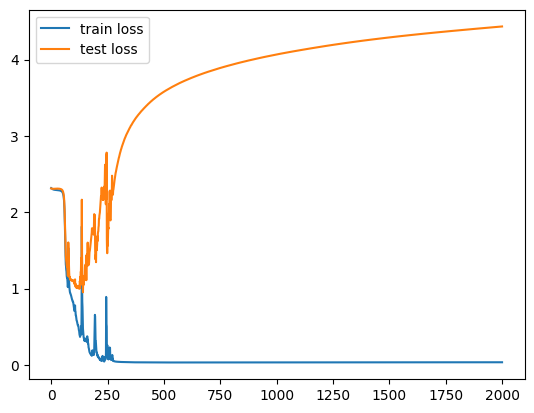
\includegraphics[width=.47\textwidth]{images/baseline_loss.png} \hfill
    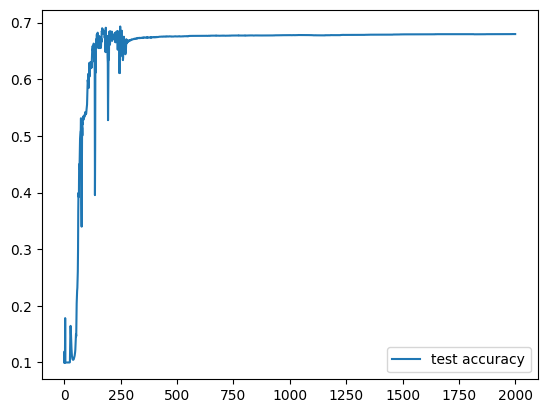
\includegraphics[width=.47\textwidth]{images/baseline_acc.png}
    \captionof{figure}{سمت راست: دقت ارزیابی مدل پایه / سمت چپ: نمودار خطای آموزش و ارزیابی (وقوع بیش‌برازش شدید)}
    \label{fig:q3_baseline}
\end{center}
}

\field{افزونگی داده‌ها (Data Augmentation) برای یادگیری تقابلی}{
برای استفاده از ۵۹۸۰۰ داده‌ی بدون برچسب، باید جفت‌های مثبت (\lr{Positive Pairs}) از تصاویر تولید می‌کردیم. بدین منظور از رویکرد افزونگی داده‌ها با اعمال تغییرات تصادفی هندسی و بصری نظیر \lr{Random Affine}، \lr{Random Perspective} و \lr{Gaussian Blur} استفاده گردید. در شکل زیر، نمونه‌هایی از جفت‌های مثبت تولید شده (مانند یک کفش یا تیشرت که با زاویه و تاری متفاوت دیده می‌شوند) قابل مشاهده است:

\vspace{0.4cm}
\begin{center}
    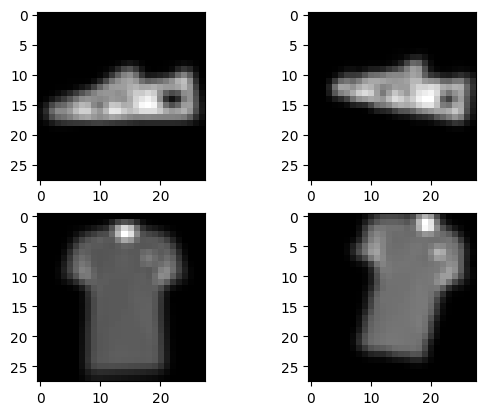
\includegraphics[width=.5\textwidth]{images/aug_pairs.png}
    \captionof{figure}{نمونه‌ای از جفت‌های مثبت تولید شده جهت آموزش بدون نظارت}
    \label{fig:q3_aug_pairs}
\end{center}
}

\field{آموزش خودنظارتی با تابع هزینه Contrastive}{
شبکه \lr{Backbone} بر روی داده‌های بدون برچسب آموزش داده شد. در این فاز از تابع هزینه \lr{Contrastive Loss} استفاده گردید تا مدل یاد بگیرد فاصله بردارهای ویژگیِ جفت‌های مثبت را کاهش و فاصله آن‌ها با سایر داده‌های درون \lr{Batch} (جفت‌های منفی) را افزایش دهد. برای بهبود همگرایی، از زمان‌بندی نمایی نرخ یادگیری (\lr{Exponential LR Scheduler}) استفاده شد. نمودارها نشان می‌دهند که تابع هزینه در طول دوره‌های آموزشی روند کاهشی مطلوبی داشته و مدل توانسته ویژگی‌های ساختاری داده‌ها را به خوبی درک کند.

\vspace{0.4cm}
\begin{center}
    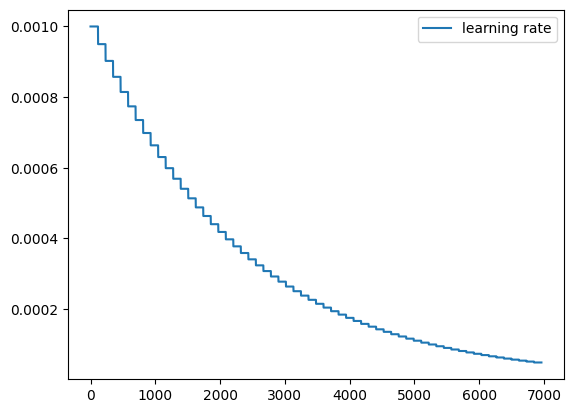
\includegraphics[width=.47\textwidth]{images/lr_schedule.png} \hfill
    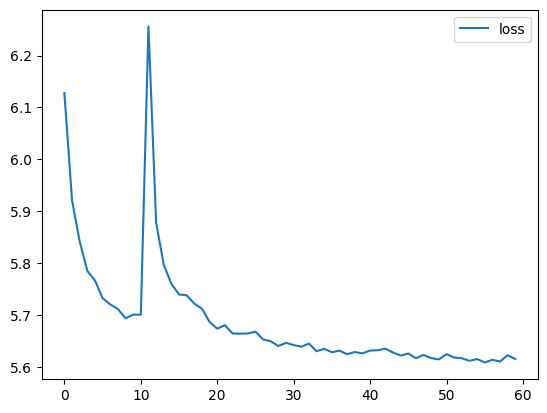
\includegraphics[width=.47\textwidth]{images/contrastive_loss.png}
    \captionof{figure}{سمت راست: روند کاهشی تابع هزینه Contrastive / سمت چپ: کاهش نمایی نرخ یادگیری}
    \label{fig:q3_ssl_training}
\end{center}
}

\field{تنظیم دقیق (Fine-Tuning) و نتیجه‌گیری نهایی}{
پس از پایان پیش‌آموزش بدون نظارت، وزن‌های آموزش‌دیده در بخش \lr{Backbone} به عنوان نقطه شروع در نظر گرفته شدند و مدل نهایی مجدداً بر روی همان ۲۰۰ داده‌ی برچسب‌دار تنظیم دقیق (\lr{Fine-tune}) گردید. 

\vspace{0.4cm}
\begin{center}
    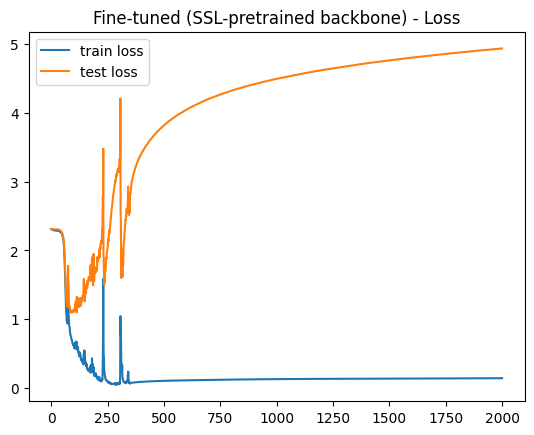
\includegraphics[width=.47\textwidth]{images/finetuned_loss.png} \hfill
    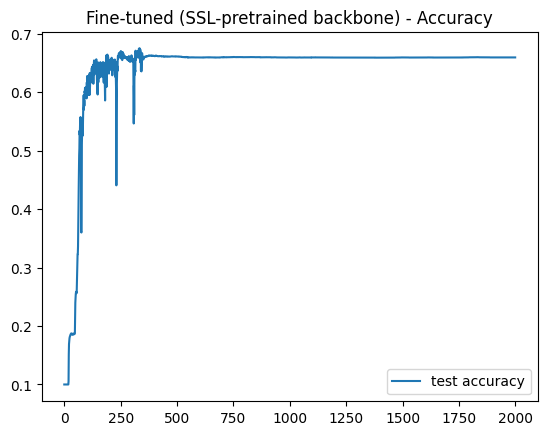
\includegraphics[width=.47\textwidth]{images/finetuned_acc.png}
    \captionof{figure}{نمودارهای خطا و دقت پس از Fine-Tuning با استفاده از وزن‌های از پیش‌آموزش‌دیده}
    \label{fig:q3_finetuned}
\end{center}
\vspace{0.4cm}

\textbf{مقایسه و جمع‌بندی نهایی:} نمودار زیر، مقایسه دقت مدل پایه (بدون پیش‌آموزش) و مدل بهره‌مند از یادگیری خودنظارتی را نشان می‌دهد. نتایج به وضوح ثابت می‌کنند مدلی که ابتدا به صورت خودنظارتی ویژگی‌های ساختاری داده‌ها را یاد گرفته باشد، در مواجهه با داده‌های به شدت محدود (تنها ۲۰۰ نمونه)، عملکرد پایدارتر و توانایی تعمیم (\lr{Generalization}) بسیار بهتری از خود نشان می‌دهد و از شدت بیش‌برازش کاسته می‌شود.

\vspace{0.4cm}
\begin{center}
    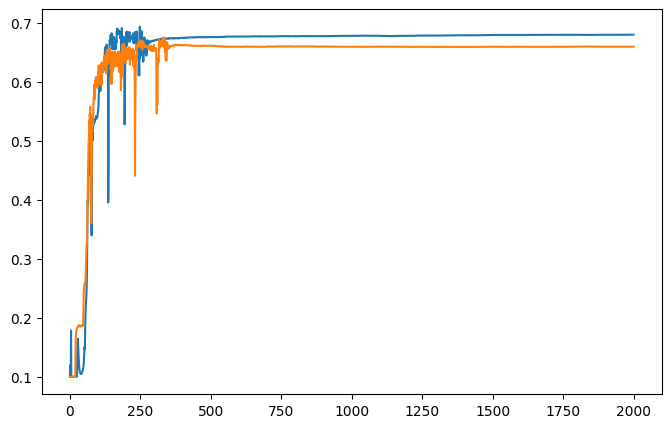
\includegraphics[width=.6\textwidth]{images/comparison_acc.png}
    \captionof{figure}{مقایسه دقت مدل پایه (آبی) با مدل خودنظارتی (نارنجی)}
    \label{fig:q3_comparison}
\end{center}
}

\end{stepbox}